\section{Surprising structures in Python}
When working so close to the specification of a language some weird or surprising structures in the language arise.
While we programmed the conversion from abstract syntax tree to a control flow graph, we had these experiences once in a while, and working with the structures has given us some insight, both in the workings of python and in the details of these interesting structures.
This section will discuss some of these experiences.

\subsection{While - else}
Normally we know \texttt{while} as a simple control structure that has a condition and a body.
The body will execute until the condition is false.
This implementation is also found in Python, but Python has an extra variant of the while loop - an else clause.
An example of a while loop with an else clause can be seen on \cref{surprise_while_else}.

\begin{figure}
  \centering
  \begin{subfigure}[b]{0.4\textwidth}
    \begin{lstlisting}[style=python]
while x < threshold:
    if invalid_value(x):
        break
    x += 1
else:
    handle_value()
    \end{lstlisting}
    \caption{A while loop with an else clause}\label{surprise_while_else}
    \end{subfigure}
  ~
    \begin{subfigure}[b]{0.4\textwidth}
      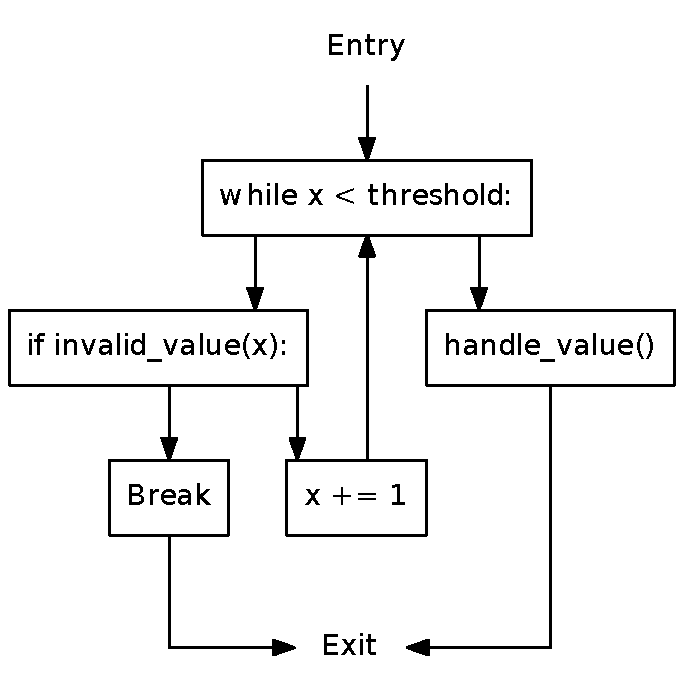
\includegraphics[scale=.4]{./figures/while_break.pdf}
      \caption{Possible flows}\label{surprise_while_else_cfg}
    \end{subfigure}
    
  \caption{An example of a while loop with a break statement}
\end{figure}


The else clause will execute when the condition is false, but if the body is exited by a \texttt{break} statement, the else clause will not be executed.
In the example in \cref{surprise_while_else}, this is being utilised to handle values that are unexpected in some way.
If that is the case, we break the body and do not execute the else clause which contains some logic for the value behaved as expected.

The \texttt{for} loop in Python also has an \texttt{else} clause which works in the same way.

\subsection{Generator expression}
The Python language has a goal of being simple, explicit and readable\citep{python_zen}.
This can often be seen in some very elegant constructions contained in the language.
One of those is the generator statement, which was discovered during the development of \pyt{}.

A generator expression is a concise notation for a common pattern: iterating over a collection of items and then performing some operation on every element\citep{python_functional}.

\begin{lstlisting}[style=python, caption={Generator expression, stripping white-space from strings}, label={generator_strip}]
strings = ['King Arthur   ', '', '   Queen Elizabeth',
           '', '   Arnold Schwarzenegger   ']

people = (line.strip() for line in strings if line != '')
\end{lstlisting}

In \cref{generator_strip} some file has been parsed into an array.
The resulting strings have some undesirable white-space, and some of the strings are even empty.
The subsequent generator expression handles both of these problems.

A generator expression consists of an expression part and a for part.
The for part is evaluated and the expression is executed on each element of the resulting iterable.
The result is a generator that contains the results.

In \cref{generator_strip} the generator iterates over the strings with the \texttt{for} statement and filters out empty strings with the \texttt{if} statement.
The resulting elements are the stripped of white-space by the initial expression.

The generator in \cref{generator_strip} can be written without using a generator expression.
This can be seen in \cref{generator_corresponding}.
The generator expression is very clear in conveying its purpose while being shorter than the ``old way''.
\begin{lstlisting}[style=python, caption={\Cref{generator_strip} implemented without using an generator expression}, label={generator_corresponding}]
for line in strings:
    if not line != '':
        yield line.strip()
\end{lstlisting}

Python contains similar constructs called the comprehensions which return a list, set or dictionary of the element instead of a generator.
This construct uses square or curly parenthesis instead of round parenthesis, but are not different in any other way.
An example of a list comprehension can be seen in \cref{listcomp}.

\begin{lstlisting}[style=python, caption={The generator from \cref{generator_strip} changed to a list comprehension}, label={listcomp}]
people = [line.strip() for line in strings if line != '']
\end{lstlisting}
